\documentclass{article}

\usepackage[english]{babel}
\usepackage[utf8]{inputenc}
\usepackage{amsmath,amssymb}
\usepackage{parskip}
\usepackage{graphicx}
\usepackage{hyperref}
% Margins
\usepackage[top=2.5cm, left=3cm, right=3cm, bottom=4.0cm]{geometry}
% Colour table cells
\usepackage[table]{xcolor}

% Get larger line spacing in table
\newcommand{\tablespace}{\\[1.25mm]}
\newcommand\Tstrut{\rule{0pt}{2.6ex}}         % = `top' strut
\newcommand\tstrut{\rule{0pt}{2.0ex}}         % = `top' strut
\newcommand\Bstrut{\rule[-0.9ex]{0pt}{0pt}}   % = `bottom' strut

%%%%%%%%%%%%%%%%%
%     Title     %
%%%%%%%%%%%%%%%%%
\title{Exercise 2 \\ Probability Theory 2020 Autumn}
\author{Hanmo Chen \\ Student ID 2020214276}
\date{\today}

\begin{document}
\maketitle
\tableofcontents
\newpage
%%%%%%%%%%%%%%%%%
%   Problem 1   %
%%%%%%%%%%%%%%%%%
\section{Problem 1}

Define the number of each dice as $X_1,X_2,X_3$ and event $A$ as $X_1>X_2>X_3$ and $B$ as $X_1,X_2,X_3$. Obviously there are $6^3 = 216$ possible combinations of $(X_1,X_2,X_3)$ with equal probability. So we just need to find the size of $A = \{(X_1,X_2,X_3)|X_1>X_2>X_3,X_1,X_2,X_3 \in \{1,2,\cdots 6\}\}$

Fix $X_1 = i$, $X_2 = j <i$, there are $j-1$ possible choices of $X_3$. So the size of $A$ is 

\begin{equation}
    \sum_{i=1}^6 \left(\sum_{j=1}^{i-1} (j-1)\right) = \sum_{i=1}^6 \left(\frac{(i-1)(i-2)}{2}\right) = 20
\end{equation}

Symmetrically, $|A| = |B| = 20$. So $P(X_1 >X_2>X_3)   = P(X_1 < X_2<X_3) = \frac{20}{216} = \frac{5}{54}$


\section{Problem 2}

\subsection{(i)}

% \paragraph*{Log Sum Inequality:} Let $ a_{1},\cdots ,a_{n}$ and $ b_{1},\cdots ,b_{n}$ be nonnegative numbers. The log sum inequality states that

% \begin{equation}
%     \sum_{i=1}^{n} a_{i} \log \frac{a_{i}}{b_{i}} \geqslant \sum_{i=1}^n a_i \log \frac{\sum_{i=1}^n a_i}{\sum_{i=1}^n b_i}
% \end{equation}

Using the Lagrange Multiplier method, 

\begin{equation}
    L = H(X) + \lambda_1(\sum_{k=1}^n p_k - 1) + \lambda_2 (\sum_{k=1}^n p_kx_k - \mu)
\end{equation}

To maximize $L$,

\begin{equation}
    \left\{
    \begin{aligned}
         &\frac{\partial L}{ \partial p_k} = 0\quad (k=1,2,\cdots,n)\\
        &\frac{\partial L}{ \partial \lambda_1} = 0 \\
        &\frac{\partial L}{ \partial \lambda_2}  = 0 
    \end{aligned}
    \right.
\end{equation}

And 

\begin{equation}
    \frac{\partial L}{ \partial p_k} = -1-\log(p_k) + \lambda_1 +\lambda_2 x_k = 0 \Longleftrightarrow p_k = e^{\lambda_2 x_k +\lambda_1-1} = Cr^{x_k}
\end{equation}

where $C = e^{\lambda_1 -1},r = e^{\lambda_2}$,which are constants determined by $\sum_{k=1}^n p_k =1$ and $\sum_{k=1}^n x_kp_k =\mu$.

\subsection{(ii)}

For a countable support set, let $n\to \infty$,

\begin{equation}
    L = H(X) + \lambda_1(\sum_{k=1}^{\infty} p_k - 1) + \lambda_2 (\sum_{k=1}^{\infty} p_kx_k - \mu)
\end{equation}

To maximize $L$,

\begin{equation}
    \left\{
    \begin{aligned}
         &\frac{\partial L}{ \partial p_k} = 0\quad (k=1,2,\cdots,\infty)\\
        &\frac{\partial L}{ \partial \lambda_1} = 0 \\
        &\frac{\partial L}{ \partial \lambda_2}  = 0 
    \end{aligned}
    \right.
\end{equation}

And 

\begin{equation}
    \frac{\partial L}{ \partial p_k} = -1-\log(p_k) + \lambda_1 +\lambda_2 x_k = 0 \Longleftrightarrow p_k = e^{\lambda_2 x_k +\lambda_1-1} = Cr^{x_k}
\end{equation}

where $C = e^{\lambda_1 -1},r = e^{\lambda_2}$,which are constants determined by $\sum_{k=1}^{\infty} p_k =1$ and $\sum_{k=1}^{\infty} x_kp_k =\mu$.

For the case of $x_k = k$,

\begin{equation}
    \left\{
        \begin{aligned}
            &\sum_{i=1}^{\infty} p_k = \sum_{i=1}^{\infty} Cr^k = \frac {Cr}{1-r} = 1 \\
            &\sum_{k=1}^{\infty} x_kp_k = \sum_{i=1}^{\infty} C kr^k= \frac {Cr}{(1-r)^2} = \mu 
        \end{aligned}
    \right.
\end{equation}

So $C =\mu-1, r = \frac{\mu-1}{\mu}$ and $P(X=k) = Cr^k$ is a geometric distribution.

\section{Problem 3 (Conditionally convergent series)}

\subsection{(i)}

According to Leibniz's test, $S_n = \sum_{n=1}^{\infty} \frac{(-1)^{n+1}}{n}
$ converges, thus

\begin{equation}
    \lim_{n\to\infty} S_n = \lim_{n\to \infty} S_{2n} = \lim_{n\to \infty} \sum_{k= 1}^n \frac {1}{n+k} = \lim_{n\to \infty} \frac{1}{n}\sum_{k= 1}^n \frac {1}{1+k/n} = \int_{0}^1 \frac {1}{1+x}dx = \ln 2
\end{equation}

\subsection{(ii)}

Notice that $1-\frac{1}{2}-\frac{1}{4} = \frac{1}{2} (1-\frac{1}{2})$, $\frac{1}{3}-\frac{1}{6}-\frac{1}{8} = \frac{1}{2} (\frac{1}{3}-\frac{1}{4})$ and so on. Thus,

\begin{equation}
    1-\frac{1}{2}-\frac{1}{4}+\frac{1}{3}-\frac{1}{6}-\frac{1}{8}+\frac{1}{5}-\frac{1}{10}-\frac{1}{12}+\cdots = \frac {1}{2} \sum_{n=1}^{\infty} \frac{(-1)^{n+1}}{n} = \frac {\ln 2} {2}
\end{equation}

\subsection{(iii)}
 
 $\frac 1 n > \ln (1+\frac 1 n) = \ln(n+1) - \ln(n)$, so $\sum_{k=1}^n \frac 1 k  > \ln(n+1)$, and the infinite sum converges. So the series $\frac{(-1)^{(n+1)}}{n}$ is conditionally convergent but not absolutely convergent.

\section{Problem 4}

\subsection{(i)}

For $X\sim\text{Geometric}(p)$,we have $E(X) = \frac {1} {p}$ and $E(X^2) = \frac {2-p}{p^2}$. 

Because $P(X-1=k |X>1) = P(X=k)$, 

\begin{equation}
    \begin{aligned}
        E[X^3|X>1] & = E[(X-1)^3+3(X-1)^2+3(X-1)+1 | X>1] \\
        & = E[X^3] + 3 E[X^2] + 3E[X] + 1 \\
        & = E[X^3] + \frac {6-3p}{p^2} + \frac {3} {p} +1
    \end{aligned}
\end{equation}

Also, $E[X^3] = E[X^3|X>1](1-p) + p$.

\begin{equation}
    E[X^3] = \frac{(\frac{6}{p^2}+1)(1-p)+p}{p} = \frac {6-6p+p^2} {p^3}
\end{equation}

For $E[X^4]$

\begin{equation}
    \begin{aligned}
        E[X^4 | X>1] & = E[(X-1)^4+4(X-1)^3 + 6(X-1)^2 + 4(X-1) +1  | X>1] \\
        & = E[(X-1)^4|X>1]+4 *\frac {6-6p+p^2} {p^3} + 6* \frac {2-p}{p^2} +  4 *\frac {1} {p} + 1 \\
        & = E[X^4] + \frac{24-12p+2p^2+p^3}{p^3} 
    \end{aligned}
\end{equation}

Also, $E[X^4] = E[X^4|X>1](1-p) + p$.

\begin{equation}
    \begin{aligned}
        E[X^4] = \frac{(\frac{24-12p+2p^2+p^3}{p^3} )(1-p)+p}{p} = \frac {24-36p+14p^2 - p^3}{p^4}
    \end{aligned}
\end{equation}

\subsection{(ii)}

First we prove that $E[X(X-1) \cdots(X-k)]=\lambda^{k+1}$,

\begin{equation}
    \begin{aligned}
        E[X(X-1) \cdots(X-k)] & = \sum_{n=0}^{\infty} n(n-1)\cdots(n-k) e^{-\lambda} \frac {\lambda^n}{n!} \\
        & = \sum_{n=k+1}^{\infty} n(n-1)\cdots(n-k) e^{-\lambda} \frac {\lambda^n}{n!} \\
        & = \sum_{m=0}^{\infty} m(m+1)\cdots (m+k+1)  e^{-\lambda} \frac {\lambda^{(m+k+1)}}{(m+k+1)!}\quad (m = n-k-1) \\
        & = \lambda^{k+1}\sum_{m=0}^{\infty} e^{-\lambda} \frac {\lambda^m}{m!} = \lambda^{k+1}
    \end{aligned}
\end{equation}

Thus, $E[X] = \lambda,E[X^2] = E[X(X-1)]+E[X] = \lambda^2 + \lambda$.

\begin{equation}
    \begin{aligned}
        E[X^3] & = E[X(X-1)(X-2)] +3 E[X^2] - 2E[X] \\
        & = \lambda^3 + 3(\lambda^2 + \lambda) - 2 \lambda = \lambda^3 + 3\lambda^2  + \lambda
    \end{aligned}
\end{equation}


\begin{equation}
    \begin{aligned}
        E[X^4] & = E[X(X-1)(X-2)(X-3)] +6 E[X^3] - 11E[X^2] +6 E[X] \\
        & = \lambda^4 + 6(\lambda^3 + 3\lambda^2  + \lambda) -11 (\lambda^2 + \lambda) + 6 \lambda \\
        & = \lambda^4 + 6 \lambda^3 + 7 \lambda^2+ \lambda
    \end{aligned}
\end{equation}

Note: \textit{This problem can also be solved using the moment generating function}.

\section{Problem 5}

If $\beta>1$, there must be a collision.

If $0\leqslant \beta \leqslant 1$, consider the probability that there is no collision. 

Let us start from the first person, who can choose any number($n$ choices). To avoid collision, the second person can only choose from the left $n-1$ numbers, and the third person $n-2$ and so on. So there are $n(n-1)\cdots(n-k+1)$ possible choices of numbers without collision. So the probability that a collision happens is

\begin{equation}
    P(n,k) = 1- \frac{n(n-1)\cdots(n-k+1)}{ n^k} = 1- \frac {n!}{n^k (n-k)!} 
\end{equation}

When $\beta = 1$, $P(n,k) = 1- \frac{n!}{n^n}$, using Stirling's formula $n ! \approx \sqrt{2 \pi n}\left(\frac{n}{e}\right)^{n}$, $\lim\limits_{n\to\infty}P(n,k) = 1$.



When $0 \leqslant \beta<1$, $n\to\infty$ , $k/n \to 0$, so $1-\frac i n \sim e^{-i/n}$,
\begin{equation}
    \frac{n(n-1)\cdots(n-k+1)}{ n^k} = 1(1-\frac {1}{n})\cdots(1-\frac {k-1}{n}) \approx \prod_{i=0}^{k-1} e^{-\frac i n} \approx e^{-\frac {k^2}{2n} }
\end{equation}



So $\beta_0 = \frac 1 2$.  

\begin{itemize}
    \item $\beta<\beta_0$: $\lim\limits_{n\to \infty} P(n,k) = 0$
    \item $\beta=\beta_0$: $\lim\limits_{n\to \infty} P(n,k) = \frac 1 {\sqrt{e}}$
    \item $\beta>\beta_0$: $\lim\limits_{n\to \infty} P(n,k) = 1$
\end{itemize}

\section{Problem 6}

\subsection{(i)}

Define the event $A_m$ as $\exists n$ s.t. $S_n = m$, and $f(m)=\mathbb{P}(A_m)$. 

It can be decomposed into one of those 6 situations,

\begin{enumerate}
    \item $\exists n$ s.t. $S_n = n-1$, and $X_{n+1} = 1$
    \item $\exists n$ s.t. $S_n = n-2$, and $X_{n+1} = 2$ (Note that when $X_{n+1} = 1$, it is the first situation)
    \item $\exists n$ s.t. $S_n = n-3$, and $X_{n+1} = 3$
    \item $\exists n$ s.t. $S_n = n-4$, and $X_{n+1} = 4$
    \item $\exists n$ s.t. $S_n = n-5$, and $X_{n+1} = 5$
    \item $\exists n$ s.t. $S_n = n-6$, and $X_{n+1} = 6$
\end{enumerate}

\begin{equation}
    f(m)= \mathbb{P}(A_m) =\frac 1 6 \sum_{i=1}^6 f(m-i),\quad m>6 
\end{equation}

For convenience, define $f(0) = 1$ and $f(n) = 0$ for $n<0$ so $f(m)=\frac 1 6 \sum_{i=1}^6 f(m-i)$ for $m>0$. 

The computer program in \textit{Python} is as follows.
\begin{figure}[htbp!]
    \centering
    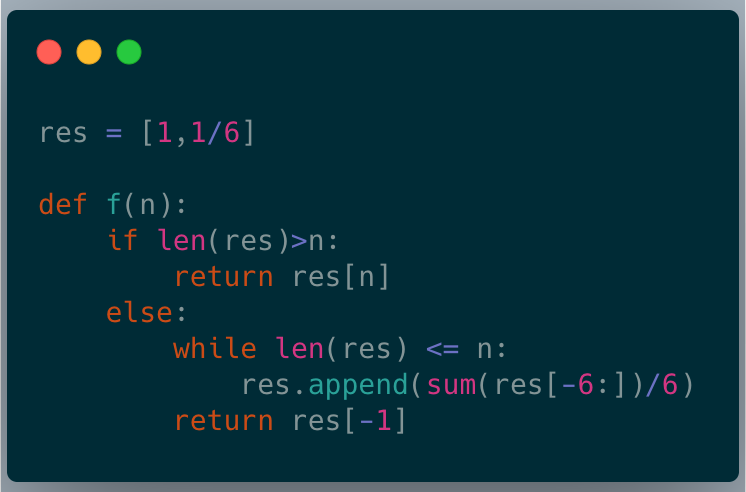
\includegraphics[scale=0.3]{carbon.png}
    \caption{Source Code to compute $f(m)$}
    \label{fig:code}
\end{figure}


\begin{equation}
    f(2020) = 0.28571428571428575
\end{equation}


\subsection{(ii)}

Consider the event $A_m^c$. It can be decomposed into one of those situations,

\begin{enumerate}
    \item $\exists n$ s.t. $S_n = n-1$, but $X_{n+1} = 2,3,4,5,6$
    \item $\exists n$ s.t. $S_n = n-2$, but $X_{n+1} = 3,4,5,6$ (Note that when $X_{n+1} = 1$, it is the first situation)
    \item $\exists n$ s.t. $S_n = n-3$, but $X_{n+1} = 4,5,6$
    \item $\exists n$ s.t. $S_n = n-4$, but $X_{n+1} = 5,6$
    \item $\exists n$ s.t. $S_n = n-5$, but $X_{n+1} = 6$
\end{enumerate}

So 

\begin{equation}\label{eq:1} 
    1-f(m) = \mathbb{P}(A_n^c) = \sum_{i=1}^5 f(m-i) \frac {6-i}{6}
\end{equation}

Suppose $f(m)$ converges as $m\to\infty$ and $p^* = \lim\limits_{m\to\infty}f(m)$, let $m\to\infty$ in the equation above (\ref{eq:1}),

\begin{equation}
    1-p^* = p^* \sum_{i=1}^5 \frac {6-i}{6} = \frac 5 2 p^*
\end{equation}

So $p^* = \frac 2 7$.


\subsection{(iii)}

Denote $a_m = \max\limits_{m-5 \leqslant n\leqslant m}f(n)$ and $b_n = \min\limits_{m-5 \leqslant n\leqslant m}f(n)$. 

\subsubsection*{Part 1}

First we prove that $a_m$ is non-increasing and $b_n$ is non-decreasing.

Because $f(m+1) = \frac 1 6 \sum\limits_{n = m-5}^{m} f(n) \leqslant \max\limits_{m-5 \leqslant n\leqslant m}f(n) = a_m$, 

$a_{m+1} = \max\limits_{m-4 \leqslant n\leqslant m+1}f(n) \leqslant \max (f(m+1),a_m) = a_m$

Symmetrically, $b_{m+1} \geqslant b_m$.

\subsubsection*{Part 2}

Because $0\leqslant b_m\leqslant b_{m+1} \leqslant a_{m+1} \leqslant a_m \leqslant 1$, $\{a_m\},\{b_m\}$ converges. 

Denote $\lim\limits_{m\to\infty} a_m = a$ and $\lim\limits_{m\to\infty} b_m = b$,  we will prove that $a=b$.

If $a>b$, let $\epsilon < \frac 1 {12}(a-b)$,  $\exists N,\forall n \geqslant N$, $a-\epsilon <a_n < a+ \epsilon,b-\epsilon <b_n < b+ \epsilon $.

Thus $\forall n \geqslant N+6, f(n) \leqslant \frac 5 6 (a+ \epsilon) + \frac 1 6 ( b+ \epsilon)\leqslant a-\epsilon$, so $a_n \leqslant a-\epsilon$, which is contradictory.

So $a=b$ and $f(m)$ converges.


\end{document}
 